\chapter{Denoising Diffusion Probabilistic Models (DDPM)}
\label{ch:ddpm}

% 1. Descriptive
Generative modeling is fundamentally an endeavor of reversing entropy. When we are presented with a dataset---images of faces, snippets of audio, or sequences of text---we are observing points drawn from a highly structured, low-entropy distribution $P_{\text{data}}$ embedded within a vast, high-entropy ambient space. The central challenge of unsupervised learning is to uncover this structure and construct a map from a simple, tractable distribution (such as a standard Gaussian) to the complex manifold of the data. 

For years, the dominant paradigms approached this problem through direct mapping or spatial bottlenecks. Generative Adversarial Networks (GANs) attempt to bridge the simple and the complex in a single, highly non-linear leap, leading to instability and mode collapse. Variational Autoencoders (VAEs) compress the data through a low-dimensional bottleneck, trading fidelity for a tractable latent space. 

Denoising Diffusion Probabilistic Models (DDPMs) take a radically different approach: instead of mapping noise to data in one step, or compressing data spatially, they operate along a \emph{temporal} axis. The core intuition is profoundly thermodynamic. If one takes a highly structured piece of data and gradually injects microscopic amounts of thermal noise over thousands of steps, the structure is slowly eroded until nothing remains but an isotropic Gaussian cloud. This is the \emph{forward process}. It is easy, deterministic, and requires no learning; it is merely the second law of thermodynamics in action, increasing the entropy of the system step by step.

The mathematical triumph of diffusion models lies in the reversal of this process. If the noise injected at each step is infinitesimally small, the reverse transitions---which must scrub away the noise to recover the previous state---take a simple functional form. They are also Gaussian. By training a neural network to approximate these small, local reverse steps, we construct a chain that slowly builds structure from chaos. We are effectively learning to run time backward, condensing a complex distribution out of a uniform fog. 

From an information-theoretic perspective, the forward process is a gradual loss of mutual information between the original signal and the noisy state. The data processing inequality guarantees that each step sheds bits of the original signal. The reverse process, parameterized by our neural network, acts as an information reservoir that optimally injects those lost bits back into the state, guided by the dataset's structural priors. This chapter rigorously formalizes this temporal destruction and reconstruction, demonstrating how it naturally leads to a variational lower bound that is both elegant and empirically powerful.

% 2. Mathematical
\section{The Diffusion Framework}

Let $\mathcal{X} = \mathbb{R}^d$ denote our continuous data space. We assume our dataset $\mathcal{D}$ consists of independent and identically distributed samples $x_0 \sim P_{\text{data}}$. Our goal is to learn a parameterized distribution $p_\theta(x_0)$ that closely approximates $P_{\text{data}}$.

\subsection{The Forward Process}

The forward diffusion process, denoted by $q$, is a Markov chain of length $T$ that progressively corrupts the data $x_0$ into a sequence of latent variables $x_1, \dots, x_T$ of the same dimensionality. The transitions are defined by a fixed variance schedule $\beta_1, \dots, \beta_T \in (0, 1)$:
\begin{equation}
    q(x_t \mid x_{t-1}) = \mathcal{N}(x_t; \sqrt{1 - \beta_t} x_{t-1}, \beta_t I)
\end{equation}
The joint distribution of the forward process is therefore:
\begin{equation}
    q(x_{1:T} \mid x_0) = \prod_{t=1}^T q(x_t \mid x_{t-1})
\end{equation}

A crucial property of this specific parameterization is that it allows us to sample $x_t$ directly from $x_0$ without simulating the intermediate steps. Let $\alpha_t = 1 - \beta_t$ and let $\bar{\alpha}_t = \prod_{s=1}^t \alpha_s$. 

\begin{lemma}[Marginal of the Forward Process]
Given the forward transition $q(x_t \mid x_{t-1})$, the marginal distribution of $x_t$ conditioned solely on $x_0$ is given by:
\begin{equation}
    q(x_t \mid x_0) = \mathcal{N}(x_t; \sqrt{\bar{\alpha}_t} x_0, (1 - \bar{\alpha}_t) I)
\end{equation}
\end{lemma}
\begin{proof}
By the reparameterization trick, we can write $x_t = \sqrt{\alpha_t} x_{t-1} + \sqrt{\beta_t} \epsilon_{t-1}$, where $\epsilon_{t-1} \sim \mathcal{N}(0, I)$. Expanding recursively, we obtain:
\begin{align*}
    x_t &= \sqrt{\alpha_t} (\sqrt{\alpha_{t-1}} x_{t-2} + \sqrt{\beta_{t-1}} \epsilon_{t-2}) + \sqrt{\beta_t} \epsilon_{t-1} \\
        &= \sqrt{\alpha_t \alpha_{t-1}} x_{t-2} + \sqrt{\alpha_t \beta_{t-1}} \epsilon_{t-2} + \sqrt{\beta_t} \epsilon_{t-1}
\end{align*}
Since the sum of two independent Gaussian variables $\mathcal{N}(0, \sigma_1^2 I)$ and $\mathcal{N}(0, \sigma_2^2 I)$ is $\mathcal{N}(0, (\sigma_1^2 + \sigma_2^2) I)$, the variance of the noise terms combines to $\alpha_t \beta_{t-1} + \beta_t = \alpha_t (1 - \alpha_{t-1}) + (1 - \alpha_t) = 1 - \alpha_t \alpha_{t-1}$. Recursively applying this to $x_0$ yields the mean $\sqrt{\bar{\alpha}_t} x_0$ and variance $(1 - \bar{\alpha}_t) I$.
\end{proof}

\begin{figure}[htbp]
\centering
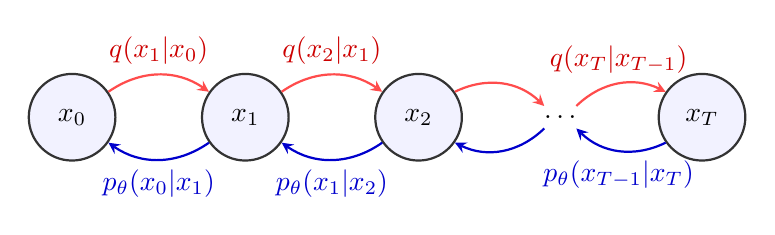
\begin{tikzpicture}[
    node distance=2.2cm,
    var/.style={circle, draw=black!80, thick, minimum size=1.1cm, fill=blue!5},
    arr/.style={->, >=stealth, thick}
]
    % Nodes
    \node[var] (x0) {$x_0$};
    \node[var, right of=x0] (x1) {$x_1$};
    \node[var, right of=x1] (x2) {$x_2$};
    \node[right of=x2, node distance=1.8cm] (dots) {$\dots$};
    \node[var, right of=dots, node distance=1.8cm] (xT) {$x_T$};

    % Forward process
    \draw[arr, bend left=35, color=red!70] (x0) to node[above, text=red!80!black] {$q(x_1|x_0)$} (x1);
    \draw[arr, bend left=35, color=red!70] (x1) to node[above, text=red!80!black] {$q(x_2|x_1)$} (x2);
    \draw[arr, bend left=35, color=red!70] (x2) to (dots);
    \draw[arr, bend left=35, color=red!70] (dots) to node[above, text=red!80!black] {$q(x_T|x_{T-1})$} (xT);

    % Reverse process
    \draw[arr, bend left=35, color=blue!80!black] (xT) to node[below, text=blue!80!black] {$p_\theta(x_{T-1}|x_T)$} (dots);
    \draw[arr, bend left=35, color=blue!80!black] (dots) to (x2);
    \draw[arr, bend left=35, color=blue!80!black] (x2) to node[below, text=blue!80!black] {$p_\theta(x_1|x_2)$} (x1);
    \draw[arr, bend left=35, color=blue!80!black] (x1) to node[below, text=blue!80!black] {$p_\theta(x_0|x_1)$} (x0);
\end{tikzpicture}
\caption{The Markov chains of the forward diffusion process $q$ and the parameterized reverse denoising process $p_\theta$. The forward process adds noise until $x_T$ is nearly an isotropic Gaussian, while the reverse process learns to systematically remove it.}
\label{fig:ddpm_markov}
\end{figure}

\subsection{The Reverse Process}
The true reverse transition $q(x_{t-1} \mid x_t)$ is intractable because it requires computing the marginal $q(x_t)$, which integrates over the entire data manifold $P_{\text{data}}$. However, if $\beta_t$ is sufficiently small, the reverse step is also approximately Gaussian. We approximate it using a neural network parameterization:
\begin{equation}
    p_\theta(x_{0:T}) = p(x_T) \prod_{t=1}^T p_\theta(x_{t-1} \mid x_t)
\end{equation}
where $p(x_T) = \mathcal{N}(x_T; 0, I)$ and $p_\theta(x_{t-1} \mid x_t) = \mathcal{N}(x_{t-1}; \mu_\theta(x_t, t), \Sigma_\theta(x_t, t))$. 

\subsection{The Variational Lower Bound}
To train the reverse process, we minimize the cross-entropy $H(P_{\text{data}}, p_\theta)$, which is equivalent to maximizing the expected log-likelihood $\mathbb{E}_{q(x_0)}[\log p_\theta(x_0)]$. Just as in VAEs, we construct an Evidence Lower Bound (ELBO).

\begin{theorem}[DDPM ELBO Decomposition]
The negative log-likelihood is bounded above by a sum of Kullback-Leibler divergences:
\begin{align}
    -\log p_\theta(x_0) &\le \mathbb{E}_{q(x_{1:T} \mid x_0)} \left[ -\log \frac{p_\theta(x_{0:T})}{q(x_{1:T} \mid x_0)} \right] \nonumber \\
    &= \mathbb{E}_{q} \Bigg[ \underbrace{D_{\text{KL}}(q(x_T \mid x_0) \parallel p(x_T))}_{L_T} \nonumber \\
    &\quad + \sum_{t=2}^T \underbrace{D_{\text{KL}}(q(x_{t-1} \mid x_t, x_0) \parallel p_\theta(x_{t-1} \mid x_t))}_{L_{t-1}} \nonumber \\
    &\quad \underbrace{- \log p_\theta(x_0 \mid x_1)}_{L_0} \Bigg]
\end{align}
\end{theorem}

\begin{proof}
We begin by introducing the latent variables and applying Jensen's inequality:
\begin{align*}
    -\log p_\theta(x_0) &= -\log \int p_\theta(x_{0:T}) dx_{1:T} \\
                        &= -\log \int q(x_{1:T} \mid x_0) \frac{p_\theta(x_{0:T})}{q(x_{1:T} \mid x_0)} dx_{1:T} \\
                        &\le \mathbb{E}_{q(x_{1:T} \mid x_0)} \left[ -\log \frac{p_\theta(x_{0:T})}{q(x_{1:T} \mid x_0)} \right]
\end{align*}
Expanding the quotient inside the expectation using the Markov property of $q$ and $p_\theta$:
\begin{align*}
    -\log \frac{p_\theta(x_{0:T})}{q(x_{1:T} \mid x_0)} &= -\log p(x_T) - \sum_{t=1}^T \log \frac{p_\theta(x_{t-1} \mid x_t)}{q(x_t \mid x_{t-1})}
\end{align*}
By Bayes' rule, $q(x_t \mid x_{t-1}) = \frac{q(x_{t-1} \mid x_t, x_0) q(x_t \mid x_0)}{q(x_{t-1} \mid x_0)}$. Substituting this into the sum causes a telescoping cancellation:
\begin{align*}
    \log \prod_{t=1}^T \frac{q(x_t \mid x_{t-1})}{p_\theta(x_{t-1} \mid x_t)} &= \log \left( \frac{q(x_T \mid x_0)}{p(x_T)} \prod_{t=2}^T \frac{q(x_{t-1} \mid x_t, x_0)}{p_\theta(x_{t-1} \mid x_t)} \frac{1}{p_\theta(x_0 \mid x_1)} \right)
\end{align*}
Taking the expectation with respect to $q$ transforms the log-ratios into KL divergences, yielding the desired decomposition.
\end{proof}

The term $L_T$ is a constant given a fixed forward schedule, as $q(x_T \mid x_0)$ contains no learnable parameters and $p(x_T)$ is fixed. The reconstruction term $L_0$ is evaluated directly. The heavy lifting happens in the summation over $L_{t-1}$. 

Crucially, the target of our reverse process, $q(x_{t-1} \mid x_t, x_0)$, is analytically tractable.

\begin{lemma}[Tractable Reverse Conditional]
The posterior $q(x_{t-1} \mid x_t, x_0)$ is a Gaussian distribution $\mathcal{N}(x_{t-1}; \tilde{\mu}_t(x_t, x_0), \tilde{\beta}_t I)$, where:
\begin{align}
    \tilde{\mu}_t(x_t, x_0) &= \frac{\sqrt{\bar{\alpha}_{t-1}} \beta_t}{1 - \bar{\alpha}_t} x_0 + \frac{\sqrt{\alpha_t} (1 - \bar{\alpha}_{t-1})}{1 - \bar{\alpha}_t} x_t \\
    \tilde{\beta}_t &= \frac{1 - \bar{\alpha}_{t-1}}{1 - \bar{\alpha}_t} \beta_t
\end{align}
\end{lemma}
\begin{proof}
This follows directly from applying Bayes' rule to the Gaussian densities: $q(x_{t-1} \mid x_t, x_0) = \frac{q(x_t \mid x_{t-1}, x_0) q(x_{t-1} \mid x_0)}{q(x_t \mid x_0)}$. Both the numerator terms and the denominator are known Gaussians from our earlier definitions. Expanding their exponents and completing the square for $x_{t-1}$ yields the mean $\tilde{\mu}_t$ and variance $\tilde{\beta}_t$.
\end{proof}

Because both $q(x_{t-1} \mid x_t, x_0)$ and $p_\theta(x_{t-1} \mid x_t)$ are Gaussian, the KL divergence in $L_{t-1}$ has a closed-form expression. If we fix the variance $\Sigma_\theta(x_t, t) = \tilde{\beta}_t I$ (or alternatively $\beta_t I$), the KL divergence minimizes the Euclidean distance between their means:
\begin{equation}
    D_{\text{KL}}(q \parallel p_\theta) = \frac{1}{2 \tilde{\beta}_t} \| \tilde{\mu}_t(x_t, x_0) - \mu_\theta(x_t, t) \|^2 + C
\end{equation}

By reparameterizing $x_0$ in terms of $x_t$ and the sampled noise $\epsilon \sim \mathcal{N}(0, I)$, we can train the network $\epsilon_\theta(x_t, t)$ to predict the noise rather than the mean. This leads to the simplified objective widely used in practice:
\begin{equation}
    \mathcal{L}_{\text{simple}}(\theta) = \mathbb{E}_{t, x_0, \epsilon} \left[ \| \epsilon - \epsilon_\theta(x_t, t) \|^2 \right]
\end{equation}

\section{An Information-Theoretic Perspective}
The diffusion process is fundamentally about controlling information flow. Let $I(X_0; X_t)$ denote the mutual information between the pristine data distribution and the latent state at time $t$. Because $X_0 \to X_1 \to \dots \to X_T$ forms a Markov chain, the Data Processing Inequality dictates that:
\begin{equation}
    I(X_0; X_1) \ge I(X_0; X_2) \ge \dots \ge I(X_0; X_T)
\end{equation}
As $t$ increases, the differential entropy $h(X_t)$ of the marginal distribution monotonically increases, upper-bounded by the entropy of the standard normal $h(\mathcal{N}(0, I))$. The capacity of $X_t$ to act as a representation of $X_0$ decays to zero.

\begin{figure}[htbp]
\centering
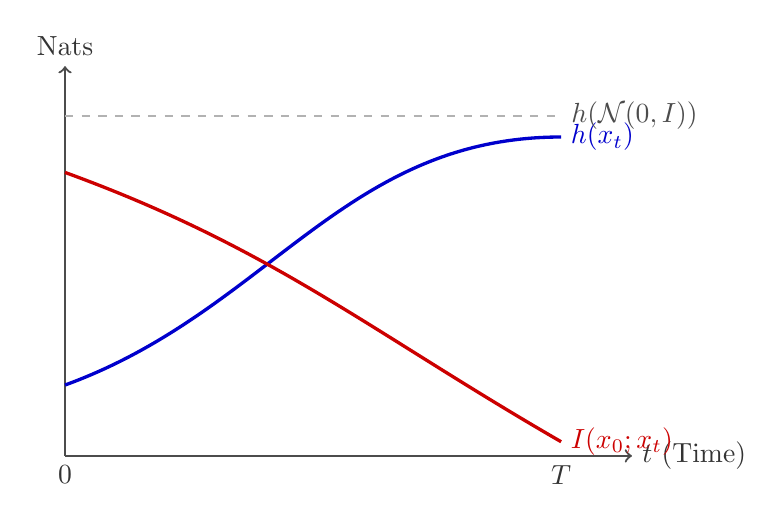
\begin{tikzpicture}[scale=0.9]
    % Axes
    \draw[->, thick, draw=black!70] (0,0) -- (8,0) node[right, text=black!80] {$t$ (Time)};
    \draw[->, thick, draw=black!70] (0,0) -- (0,5.5) node[above, text=black!80] {Nats};

    % Entropy H(X_t)
    \draw[very thick, blue!80!black] (0, 1) to[out=20, in=180] (7, 4.5);
    \node[blue!80!black, right] at (7, 4.5) {$h(x_t)$};

    % Mutual Information I(X_0; X_t)
    \draw[very thick, red!80!black] (0, 4) to[out=-20, in=150] (7, 0.2);
    \node[red!80!black, right] at (7, 0.2) {$I(x_0; x_t)$};

    % Labels
    \node[below, text=black!80] at (0,0) {$0$};
    \node[below, text=black!80] at (7,0) {$T$};
    
    % Asymptote for H
    \draw[dashed, draw=gray!60, thick] (0, 4.8) -- (7, 4.8) node[right, text=black!70] {$h(\mathcal{N}(0, I))$};
\end{tikzpicture}
\caption{Evolution of differential entropy $h(x_t)$ and mutual information $I(x_0; x_t)$ during the forward process. The Markov chain monotonically destroys information about $x_0$, causing the mutual information to decay asymptotically to zero, while the marginal entropy approaches that of an isotropic Gaussian.}
\label{fig:ddpm_mi}
\end{figure}

The reverse process $p_\theta$ is tasked with recovering this lost mutual information. Since the forward steps erase bits of structure, the neural network acts as an optimal prior that re-injects these bits, relying on the structural regularities learned from $P_{\text{data}}$ during training.

\section{Numerical Example: A 1D Diffusion Step}
To ground the continuous equations in a concrete scenario, consider a scalar random variable $x_0 = 1.0$.
Assume we are at a time step $t$ where the schedule dictates $\beta_t = 0.2$. Consequently, $\alpha_t = 0.8$. Suppose that the cumulative product $\bar{\alpha}_t = 0.64$. 

First, let us sample $x_t$ using the marginal forward distribution:
\begin{equation*}
    q(x_t \mid x_0) = \mathcal{N}(x_t; \sqrt{0.64} x_0, (1 - 0.64)) = \mathcal{N}(x_t; 0.8, 0.36)
\end{equation*}
Assume our noise sample $\epsilon = 0.5$. The latent state becomes:
\begin{equation*}
    x_t = 0.8 \times 1.0 + \sqrt{0.36} \times 0.5 = 0.8 + 0.6 \times 0.5 = 1.1
\end{equation*}

Now, suppose we want to construct the exact reverse target $q(x_{t-1} \mid x_t, x_0)$. To do this, we need $\bar{\alpha}_{t-1}$. Since $\bar{\alpha}_t = \bar{\alpha}_{t-1} \alpha_t$, we have $\bar{\alpha}_{t-1} = 0.64 / 0.8 = 0.8$. 
Applying our lemma for $\tilde{\mu}_t(x_t, x_0)$:
\begin{align*}
    \tilde{\mu}_t(1.1, 1.0) &= \frac{\sqrt{0.8} \times 0.2}{1 - 0.64} \times 1.0 + \frac{\sqrt{0.8} \times (1 - 0.8)}{1 - 0.64} \times 1.1 \\
    &\approx \frac{0.894 \times 0.2}{0.36} + \frac{0.894 \times 0.2}{0.36} \times 1.1 \\
    &\approx 0.496 + 0.546 = 1.042
\end{align*}
The variance of this transition is:
\begin{equation*}
    \tilde{\beta}_t = \frac{1 - 0.8}{1 - 0.64} \times 0.2 = \frac{0.2}{0.36} \times 0.2 \approx 0.111
\end{equation*}
The exact reverse distribution is thus tightly centered around $1.042$ with a small variance of $0.111$. The neural network's objective is to predict this mean $1.042$ (or equivalently, to predict the noise $\epsilon=0.5$ that led to $x_t$) given only $x_t = 1.1$ and the time step $t$.

\begin{horizon}
It is conjectured that the generative trajectories learned by DDPMs perfectly align with the geodesics of optimal transport maps on the Wasserstein manifold. An open question is whether we can construct an explicit cost function such that the probability flow ordinary differential equation (ODE) derived from the diffusion limit inherently minimizes this optimal transport cost, thereby achieving maximum generation efficiency without requiring adversarial entropic regularization.

Furthermore, future work might show that the intermediate representations $x_t$ of diffusion models encode a strictly ordered hierarchical disentanglement of the data manifold. If true, one could extract semantically meaningful, causally independent features at specific time scales, effectively uniting the generative synthesis power of diffusion models with the unsupervised structural decomposition previously sought by $\beta$-VAEs.
\end{horizon}

\section*{Summary}
Denoising Diffusion Probabilistic Models (DDPM) construct generative models by sequentially destroying information with Gaussian noise and training a parameterized network to reverse the process. The objective naturally falls out of the Evidence Lower Bound (ELBO), which decomposes into a sum of Kullback-Leibler divergences comparing the true denoising posterior to the parameterized reverse step. By leveraging the tractability of Gaussian marginals, the loss dramatically simplifies into predicting the noise injected into the image, forging a profound link between score matching, thermodynamics, and information theory.

\section*{Exercises}
\begin{enumerate}
    \item \textbf{Marginal Proof:} Fill in the inductive steps to rigorously prove that $\mathbb{E}[x_t \mid x_0] = \sqrt{\bar{\alpha}_t} x_0$ and $\text{Var}(x_t \mid x_0) = (1 - \bar{\alpha}_t) I$.
    \item \textbf{Deriving the Posterior:} Use Bayes' rule to explicitly derive the mean $\tilde{\mu}_t(x_t, x_0)$ and variance $\tilde{\beta}_t$ for $q(x_{t-1} \mid x_t, x_0)$. Verify the algebraic steps that group the coefficients of $x_t$ and $x_0$.
    \item \textbf{Information Decay:} Assume $P_{\text{data}}$ is a Gaussian distribution $\mathcal{N}(\mu_d, \sigma_d^2 I)$. Derive an exact closed-form expression for the mutual information $I(X_0; X_t)$ as a function of time step $t$. Show mathematically that $\lim_{t \to T} I(X_0; X_t) = 0$ as $\bar{\alpha}_T \to 0$.
\end{enumerate}

% TODO-CITE: Ensure all named results are cited.
